\documentclass[a4paper,11pt,2]{article}

\usepackage[utf8]{inputenc}
\usepackage[T1]{fontenc}
\usepackage{lmodern}
\usepackage{graphicx}
\usepackage{color}
\usepackage{hyperref}
\usepackage{amsmath}
\usepackage{amsfonts}
\usepackage{epstopdf}
\usepackage[table]{xcolor}
\usepackage{listings}
\usepackage{fancyhdr}
\usepackage{geometry}

\setlength{\hoffset}{-18pt}
\setlength{\oddsidemargin}{0pt} % Marge gauche sur pages impaires
\setlength{\evensidemargin}{9pt} % Marge gauche sur pages paires
\setlength{\marginparwidth}{54pt} % Largeur de note dans la marge
\setlength{\textwidth}{481pt} % Largeur de la zone de texte (17cm)
\setlength{\voffset}{-18pt} % Bon pour DOS
\setlength{\marginparsep}{7pt} % Séparation de la marge
\setlength{\topmargin}{0pt} % Pas de marge en haut
\setlength{\headheight}{13pt} % Haut de page
\setlength{\headsep}{10pt} % Entre le haut de page et le texte
\setlength{\footskip}{27pt} % Bas de page + séparation
\setlength{\textheight}{708pt} % Hauteur de la zone de texte (25cm)

\definecolor{mygreen}{rgb}{0,0.6,0}
\definecolor{mygray}{rgb}{0.5,0.5,0.5}
\definecolor{mymauve}{rgb}{0.58,0,0.82}

\pagestyle{fancy}
\fancyhead[L]{\leftmark} % Positionne le numéro de chapitre dans le coin en haut à gauche
\fancyhead[R]{} % Rien dans l'en-tête à droite
\fancyfoot[L]{CentraleSupélec} % Le nom de ton école préférée dans le pied de page gauche
\fancyfoot[C]{\thepage}
\fancyfoot[R]{ICE P2024} % Ta promo dans le pied de page droit
\renewcommand{\footrulewidth}{0.5pt} % Largeur du trait de séparation dans le pied de page

\lstset{ 
  backgroundcolor=\color{white},   % choose the background color; you must add \usepackage{color} or \usepackage{xcolor}; should come as last argument
  basicstyle=\footnotesize,        % the size of the fonts that are used for the code
  breakatwhitespace=false,         % sets if automatic breaks should only happen at whitespace
  breaklines=true,                 % sets automatic line breaking
  captionpos=b,                    % sets the caption-position to bottom
  commentstyle=\color{mygreen},    % comment style
  deletekeywords={...},            % if you want to delete keywords from the given language
  escapeinside={\%*}{*)},          % if you want to add LaTeX within your code
  extendedchars=true,              % lets you use non-ASCII characters; for 8-bits encodings only, does not work with UTF-8
  firstnumber=1,                % start line enumeration with line 1000
  frame=single,	                   % adds a frame around the code
  keepspaces=true,                 % keeps spaces in text, useful for keeping indentation of code (possibly needs columns=flexible)
  keywordstyle=\color{blue},       % keyword style
  language=Python,                 % the language of the code
  morekeywords={*,...},            % if you want to add more keywords to the set
  numbers=left,                    % where to put the line-numbers; possible values are (none, left, right)
  numbersep=5pt,                   % how far the line-numbers are from the code
  numberstyle=\tiny\color{mygray}, % the style that is used for the line-numbers
  rulecolor=\color{black},         % if not set, the frame-color may be changed on line-breaks within not-black text (e.g. comments (green here))
  showspaces=false,                % show spaces everywhere adding particular underscores; it overrides 'showstringspaces'
  showstringspaces=false,          % underline spaces within strings only
  showtabs=false,                  % show tabs within strings adding particular underscores
  stepnumber=2,                    % the step between two line-numbers. If it's 1, each line will be numbered
  stringstyle=\color{mymauve},     % string literal style
  tabsize=2,	                   % sets default tabsize to 2 spaces
  title=\lstname                   % show the filename of files included with \lstinputlisting; also try caption instead of title
}

\graphicspath{./Images/}

\title{Compte rendu : TP Réseau d'Accès Radio}
\author{Quentin Goulas, Lucas Hocquette}
\date{}

\begin{document}

\maketitle

This report presents the scripts used and results obtained on the Lab of the Wireless Communications class, focusing on the notions of receivers. Aside from additional comments, all reported scripts are identical to the scripts provided in the Matlab Live Script document provided as support. All plots are direct outputs from each script.

Ce rapport présente les scripts utilisés et les résultats obtenus durant le Travail Pratique de Réseau d'Accès Radio. Mis à part des commentaires additionnels, tous les scripts présentés dans ce document sont identiques aux scripts fournis dans le Jupyter Notebook en guise de support. Tous les graphes sont des outputs directs des scripts fournis.

\paragraph{Librairies requises}

\begin{center}
\begin{lstlisting}
import numpy as np
import matplotlib.pyplot as plt
\end{lstlisting}
\end{center}

\section{Capacité d'un système CDMA}
\paragraph{1} On définit la fonction \verb+sample_users+ qui prend en entrée un nombre d'utilisateurs $K$ et un rayon $R$, et retourne les positions de $K$ utilisateurs uniformément répartis dans un cercle de rayon $R$.

\begin{center}
\begin{lstlisting}
def sample_users(K,R):
    v = np.random.uniform(low=0,high=R**2,size=K)
    theta = np.random.uniform(low=0,high=2*np.pi,size=K)
    r = np.sqrt(v)
    x,y = r*np.cos(theta), r*np.sin(theta)
    return x,y
\end{lstlisting}
\end{center}

On obtient les échantillonnages présentés en figure \ref{fig:sample}.

\paragraph{2}
\begin{center}
\begin{lstlisting}
r = 1
W = 3.84*10**6
theta = 0.4
sigma2 = 10**(-104/10)*1e-3
P = 10**(40/10)*1e-3

def measure_achievement_ratio(K,R,gamma,n_avg=1):
    x,y = sample_users(K,r)
    d = np.sqrt(x**2+y**2)
    L = -128.1 - 37.6*np.log10(d)
    l = 10**(L/10)
    history = np.zeros(n_avg)
    for i in range(n_avg):
        h = np.random.exponential(0.5,K)
        g = l*h
        p = P/K
        SINR = W/R*p*g/(theta*(K-1)*p*g+sigma2)
        history[i] = np.mean(SINR>=gamma)

    return history

print(f'The percentage of users for which the decoding condition is satisified is : {measure_achievement_ratio(20,32*1e3,10**(7/10))[0]*100}%')
\end{lstlisting}
\end{center}

Avec la configuration donnée, 100\% des utilisateurs satisfont la condition.

\begin{figure}[h]
\centering
\begin{tabular}{cc}
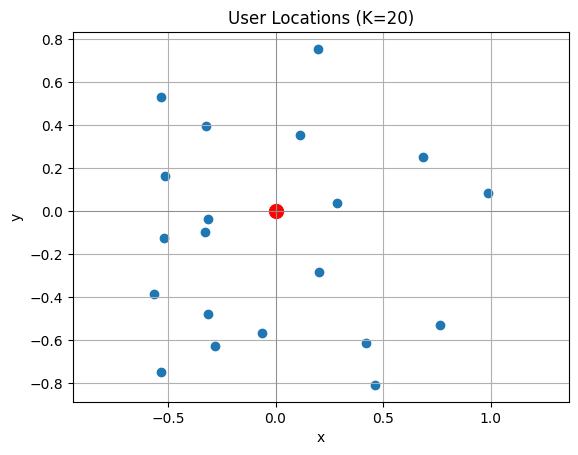
\includegraphics[width =0.4\linewidth]{./Images/k20.png} & 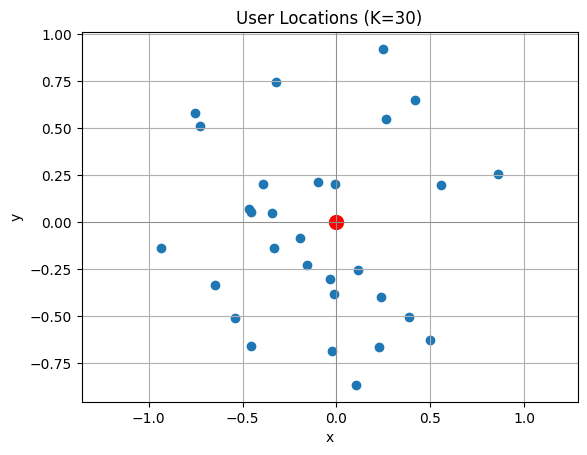
\includegraphics[width =0.4\linewidth]{./Images/k30.png}\\
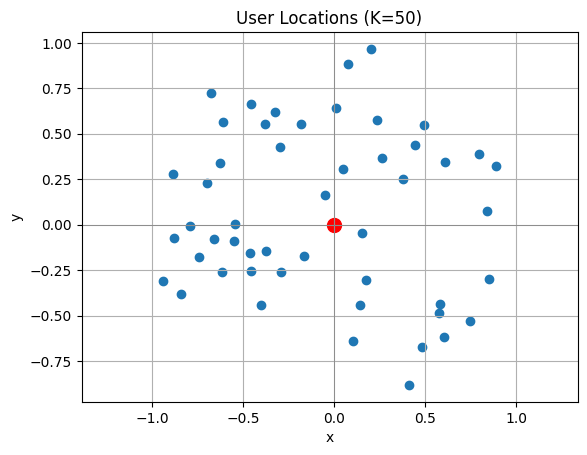
\includegraphics[width =0.4\linewidth]{./Images/k50.png} & 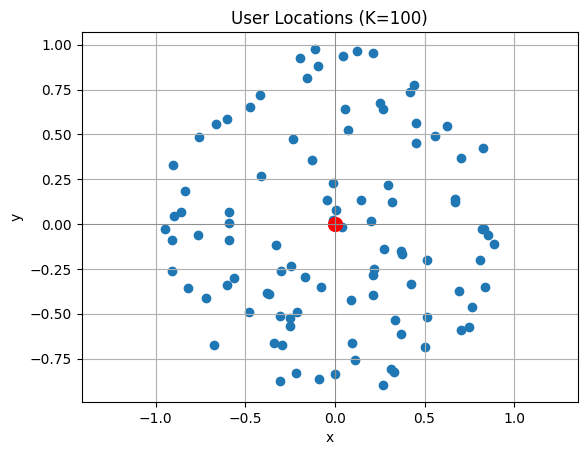
\includegraphics[width =0.4\linewidth]{./Images/k100.png}
\end{tabular}
\caption{Exemples d'échantillonnages de positions utilisateurs pour 20, 30, 50 et 100 utilisateurs}
\label{fig:sample}
\end{figure}

\paragraph{3 et 4}
\begin{center}
\begin{lstlisting}
	achievement_ratio = measure_achievement_ratio(20,32*1e3,10**(7/10),100)
	print(f'delta = {np.mean(achievement_ratio)*100}%')
\end{lstlisting}
\end{center}

On obtient des résultats de 97.95\% et 98.1\%.

\paragraph{5}
\begin{center}
\begin{lstlisting}
K_values = np.array(range(1,100))
deltas = np.zeros(len(K_values))

for i,K in enumerate(K_values) :
    ach_rat = measure_achievement_ratio(K,32*1e3,10**(7/10),100)
    deltas[i] = np.mean(ach_rat)

print(deltas)
print(f'The maximum number of users on the network is {K_values[np.sum(deltas>=0.9)]}')

plt.plot(K_values,deltas)
plt.title('Condition achievement rate by the number of users')
plt.xlabel('Number of users')
plt.ylabel('Proportion of users over SINR threshold')
plt.axhline(0.9,color='0')
plt.axvline(K_values[np.sum(deltas>=0.9)],color='0')
plt.show()
\end{lstlisting}
\end{center}
Le nombre maximal d'utilisateurs obtenu est 43, comme nous pouvons le voir en figure \ref{fig:I5}.

\begin{figure}[h]
\centering
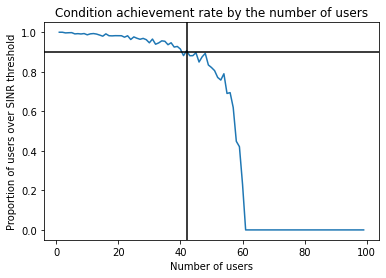
\includegraphics[width=0.7\linewidth]{./Images/I-5.png}
\caption{Proportion d'utilisateurs satisfaisant la condition de SINR en fonction du nombre total d'utilisateurs}
\label{fig:I5}
\end{figure}

\section{Contrôle de puissance uplink d'un système CDMA}
\paragraph{1.a} Nous renvoyons à la question 1 de la partie 1 pour cette question.

\paragraph{1.b} On utilise le script suivant pour obtenir le nombre maximal d'utilisateurs tel que $\rho(F)<1$ soit toujours vérifée. On rappelle, la forme de la matrice F :
$$ 
F = \begin{pmatrix} 
        0 & \frac{g_2}{R_1g_1} & \cdots & \frac{g_k}{R_1g_1} \\
        \frac{g_1}{R_2g_2} & 0 & \ddots & \vdots \\
        \vdots & \ddots & \ddots & \vdots \\
        \frac{g_1}{R_kg_k} & \cdots & \cdots & 0
    \end{pmatrix}       
$$

\begin{center}
\begin{lstlisting}
K = np.array(range(10,100,2), dtype=np.int32)
R = 1
r1,r2 = 15*1e3,32*1e3
W = 3.84*10**6
theta = 0.4
gamma1, gamma2  = 10**(5/10), 10**(7/10)
Rho = np.array([])

def generate_F(k,R,r1,r2,gamma1,gamma2,W,theta):
    x,y = sample_users(k,R)
    r = np.concatenate((r1*np.ones(k//2),r2*np.ones(k//2)))
    gamma = np.concatenate((gamma1*np.ones(k//2),gamma2*np.ones(k//2)))
    lamda = 0.5
    h = np.random.exponential(1/lamda,k)
    d = np.sqrt(x**2+y**2)
    L = -128.1 - 37.6*np.log10(d)
    l = 10**(L/10)
    g = l*h
    G1,G2 = np.meshgrid(gamma*r*g,g)
    F = (theta/W)*G1 / G2
    F[np.eye(k,dtype=bool)] = 0
    return F, r, gamma, g

for k in K:
    F,_,_,_ = generate_F(k,R,r1,r2,gamma1,gamma2,W,theta)
    rho = np.max(np.abs(np.linalg.eigvals(F)))
    Rho = np.append(Rho,rho)

Kmax = np.max(K[Rho<1])
print(Kmax)
\end{lstlisting}
\end{center}

On obtient un nombre maximum d'utilisateurs à 92.

\paragraph{1.c} Nous calculons l'allocation de puissance optimale par une simple inversion matricielle :
\begin{center}
\begin{lstlisting}
k = Kmax

x,y = sample_users(k,R)
r = np.concatenate((r1*np.ones(k//2),r2*np.ones(k//2)))
gamma = np.concatenate((gamma1*np.ones(k//2),gamma2*np.ones(k//2)))
lamda = 0.5
h = np.ones(k)
h = np.random.exponential(1/lamda,k)
d = np.sqrt(x**2+y**2)
L = -128.1 - 37.6*np.log10(d)
l = 10**(L/10)
g = l*h
G1,G2 = np.meshgrid(gamma*r*g,g)
F = (theta/W)*G1 / G2
F[np.eye(k,dtype=bool)] = 0

sigma2 = 10**(-104/10)/1000
b = sigma2*(1/(3.84*10**6))*r*gamma/g
P =  np.linalg.inv(np.eye(k) - F)@b

print(10*np.log10(P*1000)) # display the power allocation in dBm

def SINR(W,R,P,G,theta,sigma2):
    alpha = W/R
    pg = P*G
    p,_ = np.meshgrid(P,P)
    p[np.eye(len(p),dtype=bool)] = 0
    sm = np.sum(p,axis=1)*G
    return alpha*pg/(theta*sm+sigma2)

plt.hist(10*np.log10(P*1000))
plt.title('Power allocation distribution')
plt.ylabel('Number of users')
plt.xlabel('P (dBm)')
plt.show()
\end{lstlisting}
\end{center}

Ce qui nous donne la distribution de puissance en figure \ref{fig:II1c}
\begin{figure}[h]
\centering
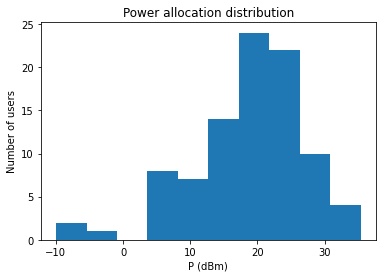
\includegraphics[width=0.7\linewidth]{./Images/II-1c.png}
\caption{Allocation de puissance optimale}
\label{fig:II1c}
\end{figure}

\paragraph{1.d} Résoudre le problème comme 1.c peut être très coûteux en calcul puisqu'il demande une inversion matricielle. Pour raccourcir le temps de calcul, nous implémentons une prémière méthode itérative pour arriver à l'allocation optimale.
\begin{center}
\begin{lstlisting}
K_list = np.array(range(10,Kmax,2), dtype=np.uint32)
epsilon = 0.1
iteration_list = np.zeros(len(K_list))

for idx in range(len(K_list)):
    k = K_list[idx]
    p = np.ones(k)
    new_p = np.ones(k)*0.1
    num_iteration = 0
    _, r, gamma, g = generate_F(k,R,r1,r2,gamma1,gamma2,W,theta)
    while not np.all(np.abs(p - new_p) < epsilon):
        p = new_p
        pg = p*g
        pg1,_ = np.meshgrid(pg,pg)
        pg1[np.eye(len(pg),dtype=bool)] = 0
        sm = np.sum(pg1,axis=1)
        new_p = (r*gamma*(theta*sm + sigma2))/(W*g)
        num_iteration += 1
    iteration_list[idx] = num_iteration
    print(f"k={k}, num_iteration={num_iteration}")

plt.plot(K_list, iteration_list, marker='o')
plt.xlabel('Number of Users (k)')
plt.ylabel(f'Number of Iterations with epsilon={epsilon}')
plt.title('Number of Iterations vs Number of Users')
plt.grid(True)
plt.show()
\end{lstlisting}
\end{center}

Ceci nous permet d'obtenir le nombre d'itérations avant convergence de l'algorithme en fonction du nombre d'utilisateurs, visible en figure \ref{fig:II1d}.
\begin{figure}[h]
\centering
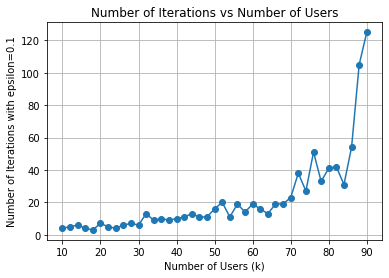
\includegraphics[width=0.7\linewidth]{./Images/II-1d.png}
\caption{Nombre d'itérations avant convergence de l'algorithme en fonction du nombre d'utilisateurs}
\label{fig:II1d}
\end{figure}

\paragraph{1.e} On implémente une deuxième méthode itérative pour résoudre le problème d'allocation.
\begin{center}
\begin{lstlisting}
def iterativeE(gamma,beta,tol,seed):
    p=seed.copy()
    p_old = np.inf*np.ones_like(p)
    iter = 0
    while np.sum(abs(p-p_old))>=tol:
        p_old = p.copy()
        sinr = SINR(W,r,p,g,theta,sigma2)
        p = (1-beta)*p + beta*gamma/sinr*p
        iter +=1
    return p, iter

Beta = np.arange(0.1,1,0.05)
Niter = np.zeros_like(Beta)
_, r, gamma, g = generate_F(Kmax,R,r1,r2,gamma1,gamma2,W,theta)

seed = np.ones(Kmax)
for b in range(len(Beta)):
    p,iter = iterativeE(gamma,Beta[b],1e-3,seed)
    Niter[b] = iter

print(Niter)

plt.plot(Beta,Niter)
plt.title('Number of iterations before convergence by beta')
plt.xlabel('Beta')
plt.ylabel('Number of iterations')
\end{lstlisting}
\end{center}

On considère cette fois le nombre d'itérations avant convergence de l'algorithme en fonction du paramètre $\beta$, avec $K_{max}=92$ utilisateurs. On obtient la courbe en figure \ref{fig:II1e}. On voit très clairement qu'avec un $\beta$ proche de 1, le nombre d'itérations nécessaire est considérablement plus faible qu'avec $\beta$ proche de 0.

\begin{figure}[h]
\centering
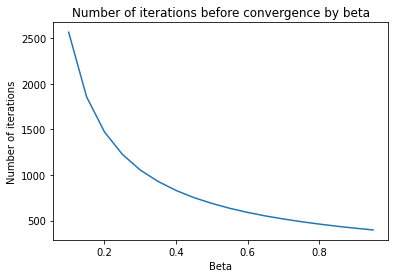
\includegraphics[width=0.7\linewidth]{./Images/II-1e.png}
\caption{Nombre d'itérations avant convergence en fonction de $\beta$}
\label{fig:II1e}
\end{figure}

\paragraph{1.f} On implémente la méthode proposée dans l'énoncé :
\begin{center}
\begin{lstlisting}
def iterativeF(gamma,alpha,tol,seed,maxIter):
    p = seed.copy()
    p_old = np.inf*np.ones_like(p)
    iter = 0
    while (np.sum(abs(p-p_old))>=tol) & (iter<maxIter):
        p_old = p.copy()
        sinr = SINR(W,r,p,g,theta,sigma2)
        p[sinr<gamma] = alpha*p_old[sinr<gamma]
        p[sinr>gamma] = p_old[sinr>gamma]/alpha
        iter +=1
    return p, iter

Alpha = 10**(np.linspace(0.25,1.5,7)/10)
Niter = np.zeros_like(Alpha)
_, r, gamma, g = generate_F(Kmax,R,r1,r2,gamma1,gamma2,W,theta)

seed = np.ones(Kmax)
for a in range(len(Alpha)):
    p,iter = iterativeF(gamma,Alpha[a],1e-3,seed,5e3)
    Niter[a] = iter

print(Niter)
\end{lstlisting}
\end{center}

Nous constatons que, pour les valeurs d'$\alpha$ proposées, l'algorithme atteint systématiquement le nombre maximum d'itérations, fixé à 5000 itérations.

\paragraph{1.g} A l'aide du script suivant : nous implémentons la nouvelle méthode itérative proposée.
\begin{center}
\begin{lstlisting}
def iterativeG(gamma,alpha,tol,maxIter):
    p = np.ones(Kmax)
    p_old = np.inf*np.ones_like(p)
    iter = 0
    while (np.sum(abs(p-p_old))/Kmax>=tol) & (iter<maxIter):
        p_old = np.copy(p)
        sinr = SINR(W,r,p,g,theta,sigma2)
        p[sinr > alpha*gamma*p_old] = p_old[sinr > alpha*gamma*p_old]/alpha
        p[sinr < gamma*alpha**(-1)] = p_old[sinr < gamma*alpha**(-1)]*alpha
        iter += 1
    return p, iter

Alpha = 10**(np.linspace(0.25,1.5,7)/10)
#Alpha = [10**(0.25/10), 10**(0.25/10), 10**(0.25/10)]
Niter = np.zeros_like(Alpha)
_, r, gamma, g = generate_F(Kmax,R,r1,r2,gamma1,gamma2,W,theta)
epsilon = 5e-3

for a in range(len(Alpha)):
    p_alpha,iter = iterativeG(gamma,Alpha[a],epsilon,5e3)
    Niter[a] = iter

print(Niter)
\end{lstlisting}
\end{center}

Nous constatons, encore une fois, que l'algorithme atteint systématiquement le nombre maximum d'itérations (fixé à 5000 itérations) pour toutes les valeurs d'$\alpha$ testées.

\paragraph{2.a} Cette étape revient à faire la même chose qu'en question 1.a.

\paragraph{2.b} Nous implémentons la méthode itérative vue en 1.e, avec cette fois une mise à jour du paramètre $h$ à chaque étape de l'itération.
\begin{center}
\begin{lstlisting}
def generate_F2(k,R,r1,r2,gamma1,gamma2,W,theta):
    x,y = sample_users(k,R)
    r = np.concatenate((r1*np.ones(k//2),r2*np.ones(k//2)))
    gamma = np.concatenate((gamma1*np.ones(k//2),gamma2*np.ones(k//2)))
    d = np.sqrt(x**2+y**2)
    L = -128.1 - 37.6*np.log10(d)
    l = 10**(L/10)
    return r, gamma, l

def iterativeE(gamma,beta,tol,seed,k,l,r,lim_iteration):
    p=seed.copy()
    p_old = np.inf*np.ones_like(p)
    iter = 0
    lamda = 0.5
    while lim_iteration > iter:

        h = np.random.exponential(1/lamda,k)
        g = l*h

        p_old = p.copy()
        sinr = SINR(W,r,p,g,theta,sigma2)
        p = ((1-beta)*p + p*beta*gamma/sinr)
        iter +=1
        
    return p, iter, sinr

lim_iteration = 1000
K = 10
Beta = np.arange(0.05,1,0.01)
Niter = np.zeros_like(Beta)
ach_rat = np.zeros_like(Beta)
r, gamma,l = generate_F2(K,R,r1,r2,gamma1,gamma2,W,theta)

seed = np.ones(K)
for b in range(len(Beta)):
    p,iter,sinr = iterativeE(gamma,Beta[b],1e-3,seed,K,l,r,lim_iteration)
    Niter[b] = iter
    ach_rat[b] = np.mean(sinr>=gamma)

plt.figure()
plt.plot(Beta,ach_rat)
plt.title('SINR condition achievement rate by beta')
plt.xlabel('Beta')
plt.ylabel('Proportion of users satisfying SINR condition')
\end{lstlisting}
\end{center}

Après avoir fait tourner la méthode pendant 1000 itérations pour différents $\beta$, on obtient le pourcentage d'utilisateurs satisfaisant la condition de SINR en fonction de beta disponible en figure \ref{fig:II2a}. Nous constatons, malgrès une variance très élevée, une tendance à la baisse de la proportion d'utilisateurs vérifiant la condition de SINR lorsque $\beta$ se rapproche de 1. Il faut donc faire un compromis dans le choix de $\beta$ entre performance du système lorsque le fading est stable et performance du système lorsqu'il évolue très rapidement.

\begin{figure}[h]
\centering
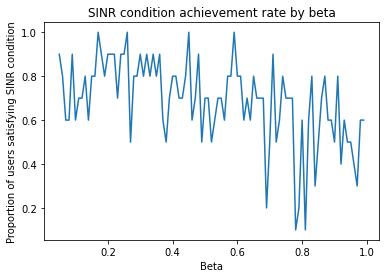
\includegraphics[width=0.7\linewidth]{./Images/II-2aii.png}
\caption{Taux de satisfaction de la condition de SINR en fonction de $\beta$}
\label{fig:II2a}
\end{figure}

\section{Comparaison entre systèmes CDMA et TDMA}
\paragraph{1} Nous réutilisons les fonctions introduites en partie 1 et reprocédons à l'analyse de la capacité du système :
\begin{center}
\begin{lstlisting}
r = 1
W = 3.84*10**6
theta = 0.4
sigma2 = 10**(-104/10)*1e-3
P = 10**(40/10)*1e-3

def measure_achievement_ratio(K,R,gamma,n_avg=1):
    x,y = sample_users(K,r)
    d = np.sqrt(x**2+y**2)
    L = -128.1 - 37.6*np.log10(d)
    l = 10**(L/10)
    history = np.zeros((n_avg,1))
    for i in range(n_avg):
        h = np.random.exponential(0.5,K)
        g = l*h
        p = P/K
        SINR = W/R*p*g/(theta*(K-1)*p*g+sigma2)
        history[i] = np.mean(SINR>=gamma)

    return history

K_values = np.array(range(1,100))
deltas = np.zeros(len(K_values))

for i,K in enumerate(K_values) :
    ach_rat = measure_achievement_ratio(K,240*1e3,10**(10/10),100)
    deltas[i] = np.mean(ach_rat)

print(deltas)
print(f'The maximum number of users on the network is {K_values[np.sum(deltas>=0.9)]}')
\end{lstlisting}
\end{center}

Nous obtenons un nombre d'utilisateurs maximum de 4.

\paragraph{2} Nous considérons cette fois un système TDMA, où un seul utilisateur a accès au réseau à la fois. Nous implémentons un algorithme d'ordonnancement de type Proportional Fairness et estimons les statistiques de débit instantané pour les utilisateurs avec le script suivant.

\begin{center}
\begin{lstlisting}
T = 1000
I = 50
gamma_i = 10**(10/10)
R_i = 240e3
L = 16                  # = W/R_i
P = 10**(40/10)*1e-3
K_list = [10, 20, 30, 40]
radius = 1
lamda = 0.5
sigma2 = 10**(-104/10)*1e-3

for K in K_list:
    try_averages = np.zeros(I)
    for idx in range(I):
        # Generate K users
        x, y = sample_users(K, radius)
        # Compute distance and pathloss effect
        d = np.sqrt(x**2+y**2)
        L = -128.1 - 37.6*np.log10(d)
        l = 10**(L/10)
        Average_rates = np.zeros(K)

        for t in range(T):
            h = np.random.exponential(1/lamda,K)
            g = l*h
            SNR_base = P*g/sigma2
            SNR = SNR_base.copy()
            C = np.ones(K)
            current_rates = np.zeros(K)
            proportional_fairness = np.zeros(K)

            for i in range(K):
                while SNR[i] > gamma_i and C[i] < 15:
                    SNR[i] = SNR_base[i]/C[i]
                    C[i] += 1
                # print(f"SNR[i] = {SNR[i]} and gamm_i = {gamma_i}")

                current_rates[i] = C[i] * R_i
                if Average_rates[i] != 0:
                    proportional_fairness[i] = np.argmax(current_rates[i]/Average_rates[i])
                else:
                    proportional_fairness[i] = np.inf
            selected_user = np.argmax(proportional_fairness)
            Average_rates[selected_user] += -(1/(t+1))*Average_rates[selected_user] + current_rates[selected_user]/(t+1)
            Average_rates[range(K) != selected_user] -= Average_rates[range(K) != selected_user]/(t+1)
        try_averages[idx] = np.mean(Average_rates)
    print(f"K={K}, Average Rate={np.mean(try_averages):.2f}, Standard Deviation={np.std(try_averages):.2f}")
\end{lstlisting}
\end{center}

Nous obtenons les résultats en table \ref{tab:III2}. Nous constatons alors que pour un débit équivalent, le système TDMA permet de servir beaucoup plus d'utilisateurs (environ 10 pour le TDMA contre 4 pour le CDMA à la question précédente). Par ailleurs, nous constantons pour un même nombre d'utilisateurs, le système TDMA peut fournir un débit plus élévé comme en comparant à la question 5 de la partie 1, où le système CDMA n'arrive à fournir que 32 kbits/s de débit pour 44 utilisateurs, où le système TDMA arrive à proposer 72 kbits/s de débit pour 40 utilisateurs (plus du double).

\begin{table}[h]
\centering
\begin{tabular}{|c|c|c|}
\hline
K & Débit instantané moyen (kbit/s) & Ecart-type du débit instantané (kbit/s) \\ \hline
10 & 307,5 & 50,0 \\
20 & 140,7 & 28,1 \\
30 & 98,12 & 16,1 \\
40 & 71,97 & 14,0 \\ \hline
\end{tabular}
\caption{Statistiques des débits instantanés en fonction du nombre d'utilisateurs}
\label{tab:III2}
\end{table}

\end{document}